% =========================================================================
\section{Specification Dependence of Concentration (RQ1)}
\label{sec:spec}

\subsection{Measures}
\label{sec:measures}
Both indices are computed over a set of participants with non-negative
weights $x_i$. The HHI is $\sum_i (100\,s_i)^2$ with $s_i = x_i/\sum_j x_j$,
on the $0$--$10{,}000$ scale of the U.S.\ merger guidelines. The Gini
coefficient is the standard discrete estimator over participants with
$x_i > 0$. For \emph{balance} concentration $x_i$ is the snapshot balance; for
\emph{flow} concentration $x_{i,w}$ is the total amount sent by $i$ in week
$w$, computed on the summed edge weights of Eq.~\eqref{eq:edgeweight}, and the
reported figure is the mean of the thirteen weekly values.

The merger guidelines are a reference scale, not a test we apply. They
classify the post-merger HHI of a defined relevant market: the 2010
Horizontal Merger Guidelines \cite{doj2010horizontal} called markets below
1{,}500 unconcentrated, between 1{,}500 and 2{,}500 moderately concentrated
and above 2{,}500 highly concentrated; the 2023 Merger Guidelines
\cite{doj2023merger} replaced them and define only a highly concentrated
market, with an HHI above 1{,}800. A ledger of token holders is not a
relevant market and an address is not a firm, so placing an address-level
HHI against these lines is an analogy that tells the reader the order of
magnitude, nothing more.

\subsection{One ledger, many specifications}
\label{sec:grid}
Table~\ref{tab:spec} varies one choice at a time from the main specification
(bold). Each row is defensible and several appear in published work
(Table~\ref{tab:lit}).

\begin{table*}[t]
\centering\footnotesize
\caption{Concentration of the same two ledgers under alternative
specifications. Each block varies one choice; bold is the main specification
used elsewhere in the paper. Balance rows: snapshot at block
\V{snapshot.block}. Flow rows: mean of thirteen weekly sender-side values
unless stated. ``Issuer'' is the seven LINK non-circulating-supply wallets and
the UNI governance timelock and token distributor. Entity resolution merges
addresses whose labels share an operator name in the archived compilation and
leaves unlabelled addresses separate, so it is a lower bound. The airdrop and
zero-value rows change the transfer records only and therefore leave
all-holder balance figures unchanged. Holders retained of \V{link.holders} (LINK) and \V{uni.holders} (UNI): transfer-active \V{link.nh.active} and \V{uni.nh.active}; airdrop kept \V{link.nh.active_noair} and \V{uni.nh.active_noair}; dust floor \V{link.n.dust} and \V{uni.n.dust}; value floor \V{link.n.value} and \V{uni.n.value}. \textsuperscript{a}Zero-value transfers removed in both
active rows; on UNI the airdrop rule removes nothing, so the two coincide.}
\label{tab:spec}
\setlength{\tabcolsep}{5pt}
\begin{tabular}{@{}llrrrr@{}}
\toprule
& & \multicolumn{2}{c}{LINK} & \multicolumn{2}{c}{UNI} \\
\cmidrule(lr){3-4}\cmidrule(l){5-6}
Choice & Specification & HHI & Gini & HHI & Gini \\
\midrule
\multicolumn{6}{@{}l}{\emph{Balance concentration}} \\
Holder population & \textbf{All positive balances} & \textbf{\V{link.hhi.all}} & \textbf{\V{link.gini.all}} & \textbf{\V{uni.hhi.all}} & \textbf{\V{uni.gini.all}} \\
 & Transfer-active, cleaned & \V{link.hhi.active} & \V{link.gini.active} & \V{uni.hhi.active} & \V{uni.gini.active} \\
 & Transfer-active, airdrop transfers kept\textsuperscript{a} & \V{link.hhi.active_noair} & \V{link.gini.active_noair} & \V{uni.hhi.active_noair} & \V{uni.gini.active_noair} \\
 & Balance $\geq$ 0.01 tokens (dust floor) & \V{link.hhi.dust} & \V{link.gini.dust} & \V{uni.hhi.dust} & \V{uni.gini.dust} \\
 & Balance $\geq$ USD 100 (value floor) & \V{link.hhi.value} & \V{link.gini.value} & \V{uni.hhi.value} & \V{uni.gini.value} \\
\addlinespace[2pt]
Address type & \textbf{All addresses} & \textbf{\V{link.hhi.all}} & \textbf{\V{link.gini.all}} & \textbf{\V{uni.hhi.all}} & \textbf{\V{uni.gini.all}} \\
 & Excluding burn address & \V{link.hhi.excl_burn} & \V{link.gini.excl_burn} & \V{uni.hhi.excl_burn} & \V{uni.gini.excl_burn} \\
 & Excluding burn and issuer & \V{link.hhi.excl_issuer} & \V{link.gini.excl_issuer} & \V{uni.hhi.excl_issuer} & \V{uni.gini.excl_issuer} \\
\addlinespace[2pt]
Entity resolution & \textbf{One address, one participant} & \textbf{\V{link.hhi.all}} & \textbf{\V{link.gini.all}} & \textbf{\V{uni.hhi.all}} & \textbf{\V{uni.gini.all}} \\
 & Labelled addresses merged & \V{link.hhi.entity} & \V{link.gini.entity} & \V{uni.hhi.entity} & \V{uni.gini.entity} \\
\addlinespace[2pt]
Snapshot time & \textbf{End of window} & \textbf{\V{link.hhi.all}} & \textbf{\V{link.gini.all}} & \textbf{\V{uni.hhi.all}} & \textbf{\V{uni.gini.all}} \\
 & Extraction date (first version) & \V{link.hhi.v1export} & \V{link.gini.v1export} & \V{uni.hhi.v1export} & \V{uni.gini.v1export} \\
\midrule
\multicolumn{6}{@{}l}{\emph{Flow concentration}} \\
Temporal aggregation & \textbf{Weekly, then averaged} & \textbf{\V{link.fhhi.weekly}} & \textbf{\V{link.fgini.weekly}} & \textbf{\V{uni.fhhi.weekly}} & \textbf{\V{uni.fgini.weekly}} \\
 & Pooled over the window & \V{link.fhhi.pooled} & \V{link.fgini.pooled} & \V{uni.fhhi.pooled} & \V{uni.fgini.pooled} \\
\addlinespace[2pt]
Flow direction & \textbf{Sender side} & \textbf{\V{link.fhhi.weekly}} & \textbf{\V{link.fgini.weekly}} & \textbf{\V{uni.fhhi.weekly}} & \textbf{\V{uni.fgini.weekly}} \\
 & Receiver side & \V{link.fhhi.in} & \V{link.fgini.in} & \V{uni.fhhi.in} & \V{uni.fgini.in} \\
\addlinespace[2pt]
Entity resolution & Labelled addresses merged & \V{link.fhhi.entity} & --- & \V{uni.fhhi.entity} & --- \\
\addlinespace[2pt]
Cleaning & Airdrop and zero-value kept & \V{link.fhhi.raw} & \V{link.fgini.raw} & \V{uni.fhhi.raw} & \V{uni.fgini.raw} \\
\addlinespace[2pt]
Edge weights & Repeated pairs overwritten & \V{link.fhhi.overwrite} & \V{link.fgini.overwrite} & \V{uni.fhhi.overwrite} & \V{uni.fgini.overwrite} \\
\bottomrule
\end{tabular}
\end{table*}

\begin{figure*}[t]
  \centering
  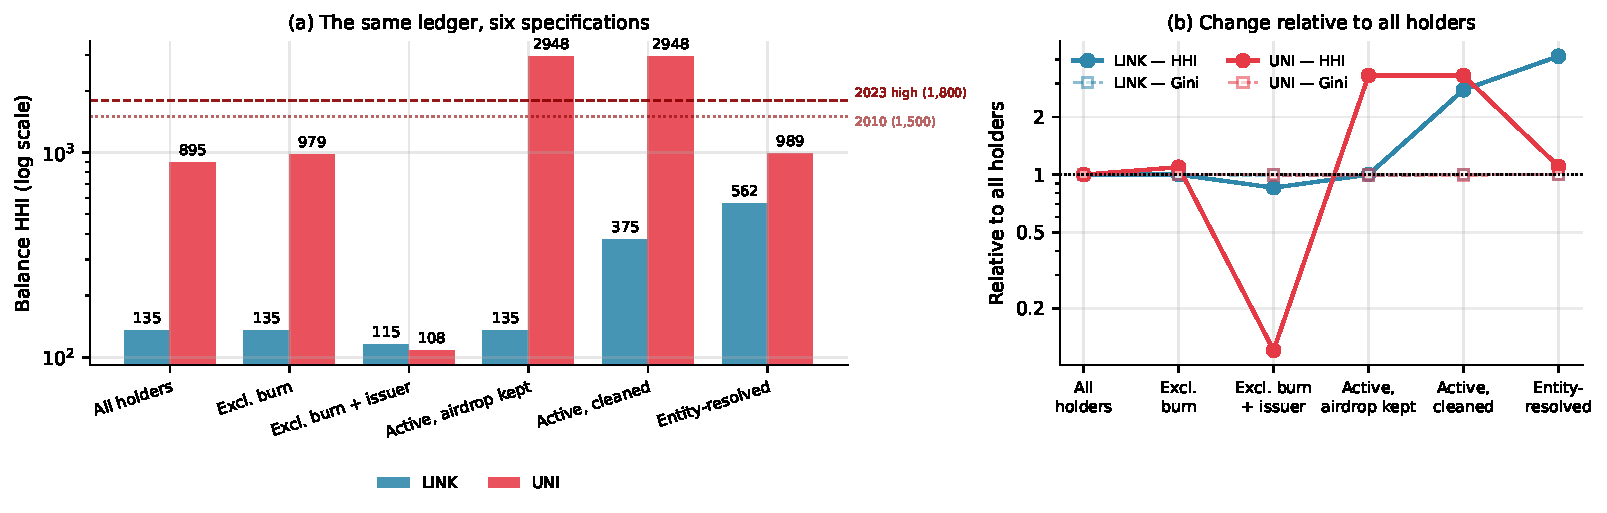
\includegraphics[width=0.95\linewidth]{fig_specification.pdf}
  \caption{Balance concentration of the same snapshot under six
  specifications. (a) HHI on a logarithmic scale; dashed line: 2023 threshold
  (1{,}800), dotted: 2010 moderate threshold (1{,}500). ``Active, airdrop
  kept'' and ``Active, cleaned'' differ only in whether the dust-airdrop
  transfers count as activity. (b) HHI and Gini relative to the all-holder
  specification: over these six specifications the HHI moves by an order of
  magnitude on UNI while the Gini stays near the unit line. The balance floors
  of Table~\ref{tab:spec}, which act on the other end of the distribution and
  move the Gini instead, are not shown.}
  \label{fig:specification}
\end{figure*}

\paragraph{Balance concentration: which end of the distribution each choice
moves}
On UNI the balance HHI runs from \V{uni.hhi.min} to \V{uni.hhi.max} across the
rows of Table~\ref{tab:spec} (Fig.~\ref{fig:specification}), a factor of \V{uni.hhi.ratio}; the lower end is
reached by excluding the burn address and the issuer, the upper end by
restricting the population to transfer-active addresses, \V{uni.active_share}
of all holders, among which the governance timelock dominates. On LINK the
range is \V{link.hhi.min}--\V{link.hhi.max}. These are the extremes of
varying one choice at a time. Over the eighteen combinations of population,
address type and entity resolution in Table~\ref{tab:combos} the UNI range
widens to \V{combo.uni.nf_hhi_min}--\V{combo.uni.nf_hhi_max}, the maximum
reached by combining the transfer-active population with entity resolution;
the LINK range is \V{combo.link.nf_hhi_min}--\V{combo.link.nf_hhi_max}. Over
the same eighteen the balance Gini moves by at most
\V{combo.link.gini_range_nofloor} on LINK and
\V{combo.uni.gini_range_nofloor} on UNI.

Varying one choice with the other two held fixed separates three kinds of
choice. \emph{Address type and entity resolution act on the top.} They
remove or merge a handful of large holders, change the HHI by up to a
factor of \V{fx.top.hhi_max} on either ledger and the Gini by at most
\V{fx.top.gini_max}. \emph{A balance floor acts on the tail.} Counting only
holdings of at least 0.01 tokens, or of at least USD~100 at the snapshot price
(\V{link.vfloor} LINK and \V{uni.vfloor} UNI, from the Chainlink price
feeds at the snapshot block), keeps \V{link.n.dust} and \V{link.n.value} of
the \V{link.holders} LINK holders and \V{uni.n.dust} and \V{uni.n.value} of
the \V{uni.holders} UNI holders. The value floor lowers the Gini by
\V{link.gini.drop_value} on LINK and \V{uni.gini.drop_value} on UNI; read as
$1-\mathrm{Gini}$, the distance from perfect inequality, that is a rise from
\V{link.omg.all} to \V{link.omg.value} (\V{link.omg.ratio}-fold) and from
\V{uni.omg.all} to \V{uni.omg.value} (\V{uni.omg.ratio}-fold). Neither
floor changes the HHI by more than \V{floor.hhi_change_max} in any cell of
the grid. \emph{Restricting to transfer-active addresses acts on both ends}:
it drops inactive large holders as well as the dormant tail, and changes the
HHI by up to a factor of \V{fx.link.activity.hhi} on LINK and
\V{fx.uni.activity.hhi} on UNI and the Gini by up to
\V{fx.link.activity.gini} and \V{fx.uni.activity.gini}. On LINK that Gini
change is more than half the value floor's (\V{fx.link.floor.gini} at most),
which is why the eighteen-cell Gini range is not small relative to the
floors. The HHI is a sum of squared shares and responds to how the largest
few participants are defined; the Gini is a function of the whole
distribution and responds to how many small holders are counted. Reporting
one does not report the other, and a population choice moves both.

For flows, averaging thirteen weekly values gives \V{link.fhhi.ratio_pooled}
(LINK) and \V{uni.fhhi.ratio_pooled} (UNI) times the HHI of the pooled 90-day
flow, because pooling averages away the week-to-week entry and exit of the
largest senders. The direction of the flow makes almost no difference.

\paragraph{Classifications that change}
Under the 2023 threshold, one row of Table~\ref{tab:spec} changes the
classification: restricting UNI to transfer-active holders, which places it
above 1{,}800 (and above 2{,}500 under the 2010 convention). No mean flow
figure on either ledger reaches 1{,}800. Among individual weeks, LINK's
largest address-level flow HHI is \V{link.fhhi.max} and its largest
entity-resolved week \V{link.fhhi.entity_max}; UNI's are \V{uni.fhhi.max} and
\V{uni.fhhi.entity_max}. Under the 2010 convention LINK's entity-resolved
maximum lies in the moderately concentrated band (above 1{,}500); under the
2023 convention, which has no moderate band, every week of both ledgers is
below the threshold.

\paragraph{The burn address raises the HHI when it is removed}
Excluding the UNI burn address, which holds \V{uni.burn_pct} of supply,
\emph{raises} the balance HHI from \V{uni.hhi.all} to \V{uni.hhi.excl_burn}.
Removing a participant with share $s_b$ removes $(100 s_b)^2$ points but
rescales every remaining squared share by $1/(1-s_b)^2$, and here the second
effect dominates.

\paragraph{Cleaning is a specification}
The transfer-active population depends on what counts as a transfer. On LINK
the dust airdrop of Section~\ref{sec:airdrop} reached most holders, so with
the airdrop transfers kept, \V{link.active_noair} addresses are
transfer-active, \V{link.nh.active_noair} of them with a positive balance, and
the HHI of those balances is \V{link.hhi.active_noair}, indistinguishable from
the all-holder figure; with them removed, \V{link.active} addresses remain
active, \V{link.nh.active} of them holders, and the HHI is
\V{link.hhi.active}. A
first-version statement that LINK's population choice was ``immaterial''
was an artefact of the airdrop. The airdrop went to existing holders rather
than creating dust-only addresses: the \V{link.airdrop_only.n} holders whose
only transfers in the window are airdrop receipts have a median balance of
\V{link.airdrop_only.med} LINK, and \V{link.airdrop_only.dust} of them hold
less than the 0.01-token dust floor. Flow concentration, being value-weighted, is
unaffected by \V{link.airdrop_total_link_short} LINK of dust.

\subsection{What the published literature uses}
\label{sec:lit}
Table~\ref{tab:lit} records the specification choices of the studies closest
to ours. None of them is wrong; they are different measurements, and their
numbers are comparable only after the choices are aligned.

\begin{table*}[t]
\centering\footnotesize
\caption{Specification choices in related studies, from the papers
themselves.}
\label{tab:lit}
\setlength{\tabcolsep}{4pt}
\begin{tabular}{@{}>{\raggedright}p{2.7cm}>{\raggedright}p{2.3cm}>{\raggedright}p{4.4cm}>{\raggedright}p{3.6cm}>{\raggedright\arraybackslash}p{3.0cm}@{}}
\toprule
Study & Quantity & Population / unit & Entity resolution & Aggregation \\
\midrule
Srinivasan \& Lee \cite{srinivasan2017quantifying} & Gini, Nakamoto & Addresses with $\geq$185 BTC or $\geq$2,477 ETH (about USD 500,000 in July 2017) & --- & Snapshot \\
Sai et al.\ \cite{sai2021wealth} & Balance Gini & All addresses with a balance (a USD 100 floor, attributed to \cite{srinivasan2017quantifying}, discussed but not applied) & ML clustering for Bitcoin only & Time series \\
Nadler \& Sch\"ar \cite{nadler2022defi} & Top-$n$, Gini & 500 largest holders & Custodial contracts mapped to beneficiaries & Snapshots \\
Lin et al.\ \cite{lin2021measuring} & Gini, entropy, Nakamoto & Mining pools & --- & Day / week / month, fixed and sliding \\
Fritsch et al.\ \cite{fritsch2024voting} & Gini, Nakamoto & Holders vs.\ delegates vs.\ voting delegates & --- & Snapshot \\
This paper & HHI, Gini, Nakamoto & All of Table~\ref{tab:spec} & Label-based, lower bound & Weekly mean and pooled \\
\bottomrule
\end{tabular}
\end{table*}

\subsection{A reporting checklist}
\label{sec:checklist}
Two on-chain concentration figures are comparable only if they agree on the
following, each of which moves at least one statistic in
Table~\ref{tab:spec}:
\begin{enumerate}
  \item the balance snapshot (block or time) and the observation window;
  \item the holder population (all positive balances, transfer-active, top
  $n$) and any balance floor;
  \item the address types excluded (burn, issuer, protocol contracts) and how
  they were identified;
  \item the unit of analysis (address or entity) and, if entities, the label
  source, its retrieval date and its coverage;
  \item for flows, the temporal aggregation and the direction;
  \item the cleaning rules (mint/burn, zero-value, spam or airdrops), with
  the number of records each removes;
  \item for anything computed on a graph, how repeated transfers between a
  pair are aggregated;
  \item for governance, whether weight is balance or delegated votes, and the
  thresholds as read from the contract.
\end{enumerate}

\subsection{Reference points}
\label{sec:benchmarks}
For orientation, Fig.~\ref{fig:hhi} places our figures beside three
reference markets whose HHI we could compute or source exactly. The national
U.S.\ deposit market, with deposits aggregated to the top-tier holding company
from the FDIC Summary of Deposits at 30 June 2026, has an HHI of
\V{bench.us_bank} \cite{fdic2026sod}; the European Central Bank reports
\V{bench.sweden} for the total assets of Swedish credit institutions in
\V{bench.sweden_year} \cite{ecb2026ssi}; and the purchase volumes of the four
largest global card networks in 2022, as published by the Nilson Report,
imply an HHI of \V{bench.cards} \cite{nilson2023issue1241}, taking shares of
the six global brands' combined volume (\V{bench.cards_top4} if the four are
taken as the whole market). National
aggregates understate the concentration of the local markets in which banks
compete, so these points indicate magnitude only. Routing on both ledgers is
of the same order as national U.S.\ deposit-taking and an order of magnitude
below card networks.

\begin{figure}[t]
  \centering
  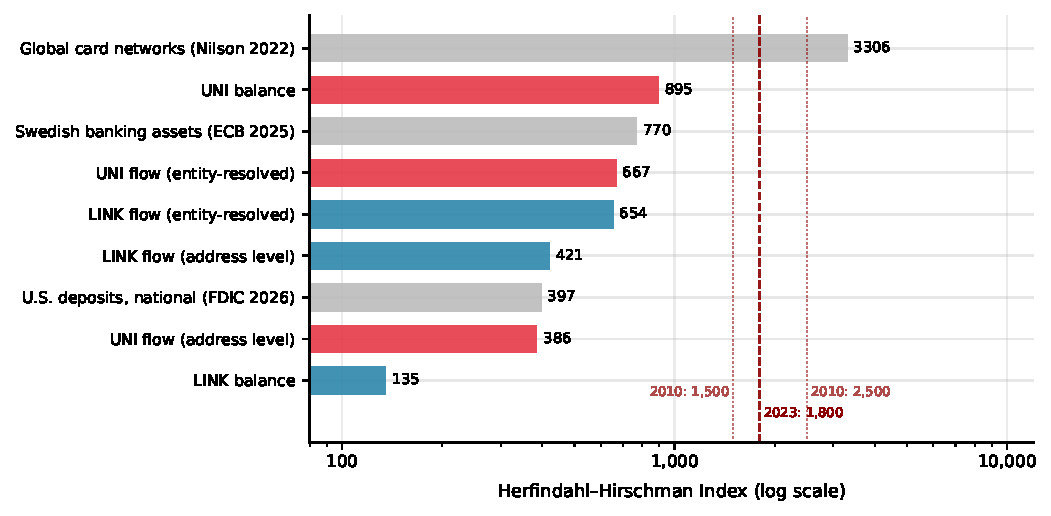
\includegraphics[width=\linewidth]{fig_hhi_benchmark.pdf}
  \caption{HHI on a logarithmic scale: balance and weekly flow concentration
  for both ledgers at address level and after label-based entity resolution,
  beside three reference markets (FDIC Summary of Deposits 2026; ECB
  structural financial indicators; Nilson Report Issue 1241). Dashed line:
  2023 Merger Guidelines threshold (1{,}800); dotted lines: 2010 thresholds
  (1{,}500 and 2{,}500). The comparison is an analogy of magnitude, not an
  application of the guidelines.}
  \label{fig:hhi}
\end{figure}

\subsection{An implementation choice that changes downstream results}
\label{sec:edgecase}
Repeated transfers between an ordered pair must be summed into one weighted
edge (Eq.~\eqref{eq:edgeweight}). Building the graph with
\texttt{networkx.from\_pandas\_edgelist(\ldots, create\_using=nx.DiGraph())}
instead keeps the last record of each pair and raises no error; node set,
edge set and degree sequence are unchanged. On the $10^{4}$ subgraphs this
discards \V{link.ew.loss_1w} (LINK) and \V{uni.ew.loss_1w} (UNI) of
transferred volume. PageRank computed the two ways has a Pearson correlation of
\V{link.ew.corr_1w} and \V{uni.ew.corr_1w}, and the fifty highest-ranked
addresses coincide in \V{link.ew.top50_1w} and \V{uni.ew.top50_1w} of fifty
positions.

We reran the whole pipeline with overwritten edges and nothing else changed
(Table~\ref{tab:edgecase}). The hidden-broker sets grow and change
membership, and the
number of brokers shared by the two ledgers goes from \V{ew.shared.main} to
\V{ew.shared.overwrite}. The classical-centrality AUC is lower with
overwritten edges, but a paired node bootstrap over pooled out-of-fold
predictions puts the difference at
\V{aci.link.cent_ow} (95\% CI \V{aci.link.cent_ow.ci}) on LINK and
\V{aci.uni.cent_ow} (\V{aci.uni.cent_ow.ci}) on UNI, so we do not read
anything into it. Weekly flow concentration moves too (\V{link.fhhi.weekly} to \V{link.fhhi.overwrite} on LINK), because
it is computed from the weighted out-degree of each weekly graph. The error is
invisible to every check that does not involve weights.

The first version of this paper attributed a further effect to this choice:
under the superseded pipeline the infrastructure cluster had a median
balance of \V{v16.core.medbal}, which had supported a contrast between the
two tokens that the corrected pipeline removed. Isolating edge aggregation
does not reproduce that result---with overwritten edges the infrastructure
cluster has a median balance of \V{ew.link.overwrite.coremedbal} against
\V{ew.link.main.coremedbal} with summed edges---so the earlier contrast
also reflected other differences between the superseded and the corrected
pipeline. We retract the attribution, not the correction: the summed
construction is the right one, and the effects in Table~\ref{tab:edgecase}
are reproducible from the archived code. We have not isolated which of the
other differences in the superseded pipeline produced the earlier contrast.

\begin{table*}[t]
\centering\small
\caption{The same pipeline with summed and with overwritten edge weights
(main cleaning specification). Rows other than the last use the $10^{4}$
subgraphs; the weekly flow HHI is computed on all cleaned transfers. Purity
ratio: neighbourhood purity of core nodes in the GraphSAGE embedding divided by
that in the structural features (\ref{app:instrument}). Brokers: set size /
overlap with the summed-edge set. AUC: fold-averaged as in
Table~\ref{tab:instrument}, and pooled over out-of-fold predictions, the
basis of the paired bootstrap in the text.}
\label{tab:edgecase}
\setlength{\tabcolsep}{3.5pt}
\begin{tabular}{@{}lcccc@{}}
\toprule
& \multicolumn{2}{c}{LINK} & \multicolumn{2}{c}{UNI} \\
\cmidrule(lr){2-3}\cmidrule(l){4-5}
& Summed & Overwritten & Summed & Overwritten \\
\midrule
Centrality AUC (fold avg.) & \V{ew.link.main.cent} & \V{ew.link.overwrite.cent} & \V{ew.uni.main.cent} & \V{ew.uni.overwrite.cent} \\
Centrality AUC (pooled) & \V{aci.link.pool.cent} & \V{aci.link.pool.cent_ow} & \V{aci.uni.pool.cent} & \V{aci.uni.pool.cent_ow} \\
GraphSAGE AUC (fold avg.) & \V{ew.link.main.gnn} & \V{ew.link.overwrite.gnn} & \V{ew.uni.main.gnn} & \V{ew.uni.overwrite.gnn} \\
Purity ratio & \V{ew.link.main.purratio} & \V{ew.link.overwrite.purratio} & \V{ew.uni.main.purratio} & \V{ew.uni.overwrite.purratio} \\
Core cluster med.\ balance & \V{ew.link.main.coremedbal} & \V{ew.link.overwrite.coremedbal} & \V{ew.uni.main.coremedbal} & \V{ew.uni.overwrite.coremedbal} \\
Brokers & \V{ew.link.main.brokers} & \V{ew.link.overwrite.brokers} / \V{ew.link.overwrite.overlap} & \V{ew.uni.main.brokers} & \V{ew.uni.overwrite.brokers} / \V{ew.uni.overwrite.overlap} \\
Weekly flow HHI & \V{link.fhhi.weekly} & \V{link.fhhi.overwrite} & \V{uni.fhhi.weekly} & \V{uni.fhhi.overwrite} \\
\bottomrule
\end{tabular}
\end{table*}
